\documentclass[a4paper,11pt]{report}
\usepackage{chuan_math_gkt}
\usetikzlibrary{angles,quotes,intersections,patterns,decorations.pathreplacing}
\chuanexamsetup

\begin{document}
\examfontsize

\examsecret{绝密$\bigstar$启用前}

\examtitle{2022年普通高等学校招生全国统一考试（天津卷）}{数\quad 学}

\noticetitle
\begin{examnotice}
\item 答卷前，考生务必将自己的姓名、准考证号填写在答题卡上。
\item 回答选择题时，选出每小题的答案后，用铅笔把答题卡上对应题目的答案标号涂黑。如需改动，用橡皮擦干净后，再选涂其他答案标号。回答非选择题时，将答案写在答题卡上。写在本试卷上无效。
\item 考试结束后，将本试卷和答题卡一并交回。
\end{examnotice}

\examsection{一、选择题：本大题共9小题，每小题5分，共45分。在每小题给出的四个选项中，只有一项是符合题目要求的。}
\begin{examquestions}

\item 设全集 $U=\{-2,-1,0,1,2\}$，集合 $A=\{0,1,2\}$，$B=\{-1,2\}$，则 $A\cap(\complement_U B)=$
\fourchoices{$\{0\}$}{$\{0,1,2\}$}{$\{-1,1,2\}$}{$\{0,-1,1,2\}$}
\item “$x$ 为整数”是“$2x+1$ 为整数”的
\twochoices{充分不必要条件}{必要不充分条件}{充分必要条件}{既不充分也不必要条件}
\item 函数 $f(x)=\dfrac{|x^2-1|}{x}$ 的图像为
\graphchoices{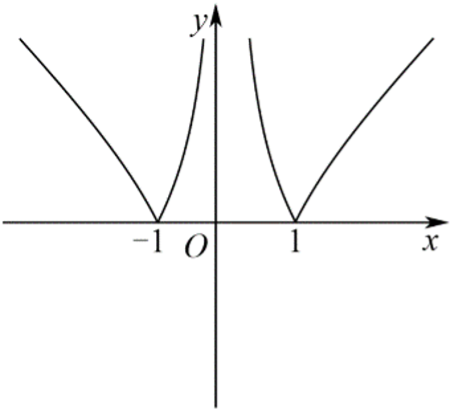
\includegraphics[width=3.6cm]{figures/2022_tj_q3_A.png}}{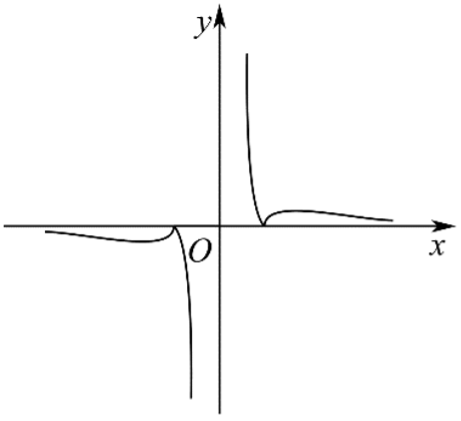
\includegraphics[width=3.6cm]{figures/2022_tj_q3_B.png}}{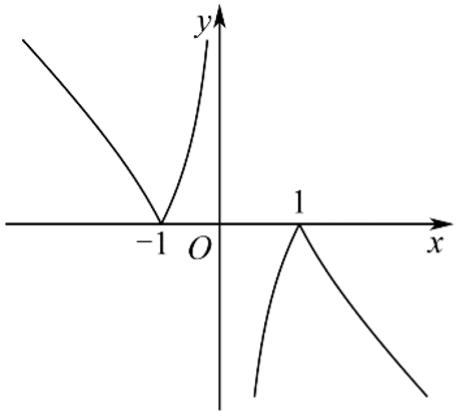
\includegraphics[width=3.6cm]{figures/2022_tj_q3_C.png}}{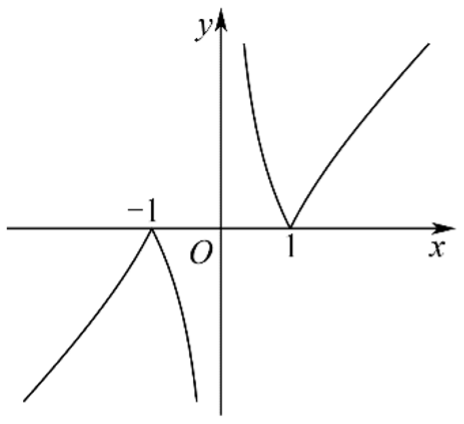
\includegraphics[width=3.6cm]{figures/2022_tj_q3_D.png}}
\newpage
\item 为研究某药品的疗效，选取若干名志愿者进行临床试验，所有志愿者的舒张压数据（单位：$\mathrm{kPa}$）的分组区间为 $[12,13),[13,14),[14,15),[15,16),[16,17]$，将其按从左到右的顺序分别编号为第一组，第二组，$\ldots$，第五组，右图是根据试验数据制成的频率分布直方图。已知第一组与第二组共有 $20$ 人，第三组中没有疗效的有 $6$ 人，则第三组中有疗效的人数为
\begin{tightcenter}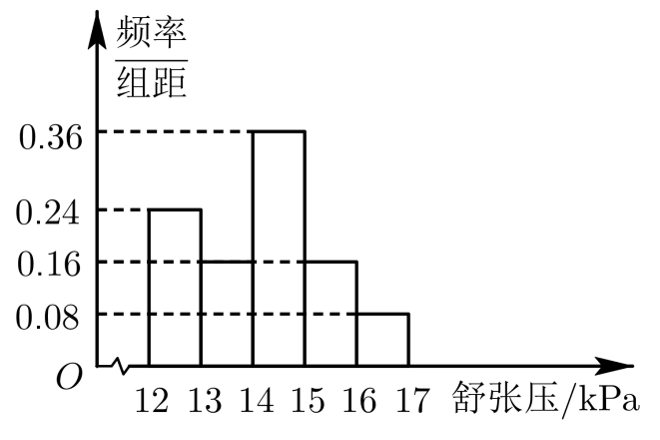
\includegraphics[width=5.5cm]{figures/2022_tj_q4.png}\end{tightcenter}
\fourchoices{$8$}{$12$}{$16$}{$18$}
\item 已知 $a=2^{0.7}$，$b=\left(\dfrac13\right)^{0.7}$，$c=\log_2\dfrac13$，则
\fourchoices{$a>c>b$}{$b>c>a$}{$a>b>c$}{$c>a>b$}
\item 化简 $(2\log_43+\log_83)(\log_32+\log_92)$ 值为
\fourchoices{$1$}{$2$}{$4$}{$6$}
\item 已知抛物线 $y^2=4\sqrt5x$，$F_1,F_2$ 分别是双曲线 $\dfrac{x^2}{a^2}-\dfrac{y^2}{b^2}=1(a>0,b>0)$ 的左、右焦点，抛物线的准线过双曲线的左焦点 $F_1$，与双曲线的渐近线交于点 $A$，若 $\angle F_1F_2A=\dfrac\pi4$，则双曲线的标准方程为
\twochoices{\tallchoice{$\dfrac{x^2}{10}-y^2=1$}}{\tallchoice{$x^2-\dfrac{y^2}{16}=1$}}{\tallchoice{$x^2-\dfrac{y^2}{4}=1$}}{\tallchoice{$\dfrac{x^2}{4}-y^2=1$}}
\item 如图，“十字歇山”是由两个直三棱柱重叠后的景象，重叠后的底面为正方形，直三棱柱的底面是顶角为 $120^\circ$，腰为 $3$ 的等腰三角形，则该几何体的体积为
\begin{tightcenter}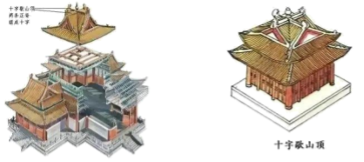
\includegraphics[width=8.0cm]{figures/2022_tj_q8.png}\end{tightcenter}
\fourchoices{$23$}{$24$}{$26$}{$27$}
\item 已知 $f(x)=\dfrac12\sin2x$，关于该函数有下列四个说法：① $f(x)$ 的最小正周期为 $2\pi$；② $f(x)$ 在 $\left[-\dfrac\pi4,\dfrac\pi4\right]$ 上单调递增；③当 $x\in\left[-\dfrac\pi6,\dfrac\pi3\right]$ 时，$f(x)$ 的取值范围为 $\left[-\dfrac{\sqrt3}{4},\dfrac{\sqrt3}{4}\right]$；④ $f(x)$ 的图象可由 $g(x)=\dfrac12\sin\left(2x+\dfrac\pi4\right)$ 的图象向左平移 $\dfrac\pi8$ 个单位长度得到。以上四个说法中，正确的个数为
\fourchoices{$1$}{$2$}{$3$}{$4$}

\end{examquestions}

\examsection{二、填空题：本大题共6小题，每小题5分，共30分。试题中包含两个空的，答对1个的给3分，全部答对的给5分。}
\begin{examquestions}[start=10]

\item 已知 $\mathrm{i}$ 是虚数单位，化简 $\dfrac{11-3\mathrm{i}}{1+2\mathrm{i}}$ 的结果为\blank。
\item $\left(\sqrt x+\dfrac3{x^2}\right)^5$ 的展开式中的常数项为\blank。
\item 若直线 $x-y+m=0(m>0)$ 与圆 $(x-1)^2+(y-1)^2=3$ 相交所得的弦长为 $m$，则 $m=$\blank。
\item $52$ 张扑克牌，没有大小王，无放回地抽取两次，则两次都抽到 A 的概率为\blank；已知第一次抽到的是 A，则第二次抽取 A 的概率为\blank。
\item 在 $\triangle ABC$ 中，$\overrightarrow{CA}=\vec a$，$\overrightarrow{CB}=\vec b$，$D$ 是 $AC$ 中点，$\overrightarrow{CB}=2\overrightarrow{BE}$，试用 $\vec a,\vec b$ 表示 $\overrightarrow{DE}$ 为\blank；若 $\overrightarrow{AB}\perp\overrightarrow{DE}$，则 $\angle ACB$ 的最大值为\blank。
\item 设 $a\in\mathbb R$，对任意实数 $x$，记 $f(x)=\min\{|x|-2,x^2-ax+3a-5\}$。若 $f(x)$ 至少有 $3$ 个零点，则实数 $a$ 的取值范围为\blank。

\end{examquestions}

\examsection{三、解答题：本大题共5小题，共75分。解答应写出文字说明、证明过程或演算步骤。}
\begin{examanswers}[start=16]

\item（14分）

在 $\triangle ABC$ 中，角 $A,B,C$ 的对边分别为 $a,b,c$。已知 $a=\sqrt6$，$b=2c$，$\cos A=-\dfrac14$。

（1）求 $c$ 的值；

（2）求 $\sin B$ 的值；

（3）求 $\sin(2A-B)$ 的值。
\newpage
\item（15分）

直三棱柱 $ABC-A_1B_1C_1$ 中，$AA_1=AB=AC=2$，$AA_1\perp AB$，$AC\perp AB$，$D$ 为 $A_1B_1$ 的中点，$E$ 为 $AA_1$ 的中点，$F$ 为 $CD$ 的中点。

\noindent\begin{minipage}[t]{0.64\linewidth}
（1）求证：$EF\parallel$ 平面 $ABC$；

（2）求直线 $BE$ 与平面 $CC_1D$ 所成角的正弦值；

（3）求平面 $A_1CD$ 与平面 $CC_1D$ 所成二面角余弦值。
\end{minipage}\hfill
\begin{minipage}[t]{0.30\linewidth}
\vspace{-1.0em}\centering
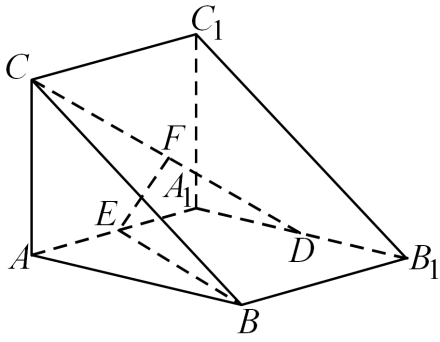
\includegraphics[width=\linewidth]{figures/2022_tj_q17.png}
\end{minipage}

\item（15分）

设 $\{a_n\}$ 是等差数列，$\{b_n\}$ 是等比数列，且 $a_1=b_1=a_2-b_2=a_3-b_3=1$。

（1）求 $\{a_n\}$ 与 $\{b_n\}$ 的通项公式；

（2）设 $\{a_n\}$ 的前 $n$ 项和为 $S_n$，求证：$(S_{n+1}+a_{n+1})b_n=S_{n+1}b_{n+1}-S_nb_n$；

（3）求 $\displaystyle\sum_{k=1}^{2n}[a_{k+1}-(-1)^ka_k]b_k$。

\item（15分）

椭圆 $\dfrac{x^2}{a^2}+\dfrac{y^2}{b^2}=1(a>b>0)$ 的右焦点为 $F$，右顶点为 $A$，上顶点为 $B$，且满足 $\dfrac{|BF|}{|AB|}=\dfrac{\sqrt3}{2}$。

（1）求椭圆的离心率 $e$；

（2）直线 $l$ 与椭圆有唯一公共点 $M$，与 $y$ 轴相交于 $N$（$N$ 异于 $M$）。记 $O$ 为坐标原点，若 $|OM|=|ON|$，且 $\triangle OMN$ 的面积为 $\sqrt3$，求椭圆的标准方程。

\item（16分）

已知 $a,b\in\mathbb R$，函数 $f(x)=e^x-a\sin x$，$g(x)=b\sqrt x$。

（1）求函数 $y=f(x)$ 在 $(0,f(0))$ 处的切线方程；

（2）若 $y=f(x)$ 和 $y=g(x)$ 有公共点，

（i）当 $a=0$ 时，求 $b$ 的取值范围；

（ii）求证：$a^2+b^2>e$。

\end{examanswers}

\end{document}
